\section{Exploratory study: Integrating the stress-buffering effect into stress prediction}
\paragraph{Stress prediction model}
To measure the effectiveness of our method for quantifying the restoring impact of positive events,
we integrate the impact of positive events into traditional stress series prediction problem,
and verify whether the restoring pattern of positive events could help improve the prediction performance.
Here we choose the SVARIMA (Seasonal Autoregressive Integrated Moving Average) algorithm \cite{Shumway2006Time},
which is proved to be suitable for teens' linear stress prediction problem \cite{Li2015Predicting},
due to the seasonality and non-stationarity of teens' stress series.
The basic stress prediction is conducted using SVARIMA approach,
in the set of stressful intervals impacted by positive events (U-SI).
Since stressor events cause the fluctuation of stress series from normal states,
%and the simple series prediction method is difficult to handle such exception.
to eliminate the interference,
we simply consider the prediction problem in those stressful intervals rather than randomly picked out stress series.
The impact of positive events are utilized as adjust values to modify the stress prediction result.
Four metrics are adopted to measure the stress forecasting problem,
where \emph{MSE}, \emph{RMSE} and \emph{MAD} measure absolute errors and \emph{MAPE} measures relative errors.
%For all real stress value $\overline{s_i}$ and predicted stress value $s_i$ in predicting sequence $<s_1,\cdots,s_n>$,
%$MSE = \frac{1}{n}\sum_{i\in[1,n]}(s_i-\overline{s_i})^2$,
%$RMSE = \frac{1}{n}\sqrt{\sum_{i\in[1,n]}(s_i-\overline{s_i})^2}$,
%$MAD = \frac{1}{n}\sum_{i\in[1,n]}|s_i-\overline{s_i}|$,
%and $MAPE = \frac{1}{n}\sum_{i\in[1,n]}{|s_i-\overline{s_i}|/s_i}$.

\begin{table*}
\caption{Compare the stress forecast performance under three restoring patterns of positive events.}
\begin{minipage}{\linewidth}
\centering
\resizebox{\textwidth}{20mm}{
\begin{tabular}{l cccc cccc cccc cccc} \\\hline\hline%\toprule
\multirow{2}{1cm}{}&\multicolumn{4}{c}{None}
    &\multicolumn{4}{c }{Positive (L)}
    &\multicolumn{4}{c }{Positive (S)}
    &\multicolumn{4}{c}{Positive (P)}\\
    &\scriptsize{MSE} &\scriptsize{RMSE} &\scriptsize{MAPE} &\scriptsize{MAD}
    &\scriptsize{MSE} &\scriptsize{RMSE} &\scriptsize{MAPE} &\scriptsize{MAD}
    &\scriptsize{MSE} &\scriptsize{RMSE} &\scriptsize{MAPE} &\scriptsize{MAD}
    &\scriptsize{MSE} &\scriptsize{RMSE} &\scriptsize{MAPE} &\scriptsize{MAD} \\\midrule					
School life
&   0.0856 	&	0.2926 	&	0.4852 	&	0.1146	&	0.0259 	&	0.1609 	&	0.2991 	&	0.0923 	
&	0.0297 	&	0.1723 	&	0.3135 	&	0.0899 	&	0.0223 	&	0.1493 	&	0.3438 	&	0.0931 	\\
Romantic
&   0.0703 	&	0.2651 	&	0.3555 	&	0.1083 	&	0.0291 	&	0.1706 	&	0.2832 	&	0.0919 	
&	0.0379 	&	0.1947 	&	0.2941 	&	0.1026 	&	0.0332 	&	0.0835 	&	0.2746 	&	0.1240 	\\
Peer relationship
&   0.2800 	&	0.5292 	&	0.3256 	&	0.1697 	&	0.3140 	&	0.5604 	&	0.3626 	&	0.1202 	
&	0.2972 	&	0.5452 	&	0.3060 	&	0.1298 	&	0.2557 	&	0.1472 	&	0.3481 	&	0.1458 	\\
Self-cognition
&   0.0445 	&	0.2110 	&	0.3066 	&	0.1895 	&	0.0345 	&	0.1857 	&	0.2721 	&	0.1653 	
&	0.0366 	&	0.1913 	&	0.2557 	&	0.0754 	&	0.0245 	&	0.0862 	&	0.2863 	&	0.1447 	\\
Family life
&   0.1602 	&	0.4002 	&	0.3291 	&	0.1587 	&	0.0889 	&	0.2982 	&	0.2891 	&	0.0944 	
&	0.0378 	&	0.1944 	&	0.2952 	&	0.0842 	&	0.1827 	&	0.0979 	&	0.3148 	&	0.1131 	\\
All	
&   0.1281 	&	0.3579 	&	0.3604 	&	0.1482	&	0.0985 	&	0.3138 	&	0.3012 	&	0.1128 	
&	0.0878 	&	0.2964 	&	0.2929 	&	0.0964 	&	0.1037 	&	0.1128 	&	0.3135 	&	0.1241 	\\ \hline\hline
\end{tabular}}
\end{minipage}\\
\begin{minipage}{\linewidth}
\centering
\resizebox{\textwidth}{20mm}{
\begin{tabular}{l cccc cccc cccc cccc} \\\hline\hline%\toprule
\multirow{2}{1cm}{}&\multicolumn{4}{c}{Positive (L\&S)}
    &\multicolumn{4}{c }{Positive (L\&P)}
    &\multicolumn{4}{c }{Positive (S\&P)}
    &\multicolumn{4}{c}{Positive (L\&S\&P)}\\
    &\scriptsize{MSE} &\scriptsize{RMSE} &\scriptsize{MAPE} &\scriptsize{MAD}
    &\scriptsize{MSE} &\scriptsize{RMSE} &\scriptsize{MAPE} &\scriptsize{MAD}
    &\scriptsize{MSE} &\scriptsize{RMSE} &\scriptsize{MAPE} &\scriptsize{MAD}
    &\scriptsize{MSE} &\scriptsize{RMSE} &\scriptsize{MAPE} &\scriptsize{MAD} \\\midrule					
School life
&	0.0283 	&	0.1682 	&	0.2934 	&	0.0824 	&	0.0261 	&	0.1616 	&	0.2770 	&	0.0768 	
&	0.0342 	&	0.1849 	&	0.2629 	&	0.0590 	&	0.0132 	&	0.1149 	&	0.2364 	&	0.0717 	\\
Romantic
&	0.0219 	&	0.1480 	&	0.2532 	&	0.0839 	&	0.0180 	&	0.1342 	&	0.2644 	&	0.0952 	
&	0.0176 	&	0.1327 	&	0.2549 	&	0.0823 	&	0.0251 	&	0.1584 	&	0.2507 	&	0.0891 	\\
Peer relationship
&	0.2361 	&	0.4859 	&	0.3182 	&	0.1300 	&	0.2349 	&	0.4847 	&	0.3283 	&	0.1189 	
&	0.2351 	&	0.4849 	&	0.3558 	&	0.1297 	&	0.2341 	&	0.4838 	&	0.3096 	&	0.1093 	\\
Self-cognition
&	0.0329 	&	0.1814 	&	0.2942 	&	0.0946 	&	0.0262 	&	0.1619 	&	0.2791 	&	0.0858 	
&	0.0245 	&	0.1565 	&	0.2740 	&	0.0945 	&	0.0144 	&	0.1200 	&	0.2580 	&	0.0739 	\\
Family life
&	0.1489 	&	0.3859 	&	0.2750 	&	0.1244 	&	0.0395 	&	0.1987 	&	0.2853 	&	0.0939 	
&	0.0484 	&	0.2200 	&	0.2946 	&	0.0992 	&	0.0378 	&	0.1944 	&	0.2645 	&	0.0848 	\\
All
&	0.0936 	&	0.3060 	&	0.2868 	&	0.1031 	&	0.0689 	&	0.2626 	&	0.2868 	&	0.0941 	&	0.0720 	&	0.2683 	&	0.2884 	&	0.0929 	&	0.0649 	&	0.2548 	&	0.2638 	&	0.0858 	\\ \hline\hline
\end{tabular}}
\begin{tablenotes}
        \footnotesize
        \item[1] $^1$ Three restoring pattern measures: 'L' represents \emph{linguistic expression}, 'S' represents \emph{stress intensity}, and 'P' represents \emph{posting behavior}.
      \end{tablenotes}
\end{minipage}
\label{tab:forecast}
\end{table*}

We integrate the impact of positive events into stress prediction.
The experimental set contains 1,914 stressful intervals under the impact of positive events (U-SI).
As shown in Table \ref{tab:forecast},
the original prediction result using only SVARIMA method
achieves 0.1281 MSE, 0.3579 RMSE, 0.3604 MAPE and 0.1482 MAD ($L = 7$, $\alpha = 0.5$).
Then we integrate the impact of each type of positive events into stress prediction.
Specifically, for positive with obvious restoring impact (under the L\&S\&P pattern),
the average stress level during historical restoring intervals are integrated to modify the result,
with adjusting the parameter $\alpha$ (details see \ref{sec:parameter}).
After the modification,
the prediction performance achieves 0.0649 MSE,	0.2548 RMSE, 0.2638 MAPE and 0.0858 MAD,
reducing the prediction errors efficiently (with MSE, RMSE, MAPE and MAD reduced by 49.34\%, 28.81\%, 26.80\% and 42.11\%, respectively).


\begin{figure*}
\centering
\caption{Teens' stress forecast performance under different lengths of predicting windows.}
\includegraphics[width=\linewidth]{figs/predictWindow2.eps}
\label{fig:length}
\end{figure*}


\paragraph{Predicting stress under different windows}
We present the prediction result under the impact of positive events under different lengths of prediction windows,
ranging from 1 to 10 days, as shown in \ref{fig:length}.
With the window length increasing,
the prediction error shows decreasing trend in all metrics.
The reason is that longer prediction window takes more previous predicted results,
and the error accumulates with more predicted values taken into the next step prediction.
Among the five dimensions of events,
the prediction for school life stress achieves the best performance.
On one side,
more positive events and stressors about school life events are detected from teens microblogs,
providing sufficient data in prediction.
On the other side,
stress coming from school life is the most common stress in the student group,
with relative stable periodicity and high frequency.


\paragraph{Contribution of each restoring measure}
We conduct experiments with different restoring patterns included respectively to show
its contribution to the impact of positive events during prediction.
Four groups of situations are considered here, as shown in Table \ref{tab:forecast},
considering
1) all the stress intensity, linguistic expression and post behavior measures (the L\&S\&P pattern),
2) any two of the three measures included (the L$|$S, L\&P, and S\&P patterns),
3) only one of the three measures included (the L, S, or P patterns),
and 4) none measure included.
We integrate the impact of positive events under the four situations into stress prediction
using the parameter $\alpha$,
as overlapping $\alpha \times S_{historical}$,
where $S_{historical}$ is the average stress level in historical restoring intervals.
The detailed adjust process of $\alpha$  is presenting in section \ref{sec:parameter}.
Here we present the prediction result when $\alpha = 0.5$ in each dimension of stress respectively.
Results show that the correlation in the L\&S\&P pattern outperforms other patterns
(0.0649 MSE, 0.2548 RMSE, 0.2638 MAPE and 0.0858 MAD),
showing the effectiveness of considering all the three correlations.

\paragraph{Parameter settings}
\label{sec:parameter}
The parameter $\alpha$ is adjusted when integrate the impact of positive events into stress prediction.
For each of the four groups of restoring patterns,
we adjust $\alpha$ in the effect of $\alpha \times L$.
We calculate the corresponding prediction result for each teen respectively,
and show the result of the whole testing group using the averaging performance.
Figure \ref{fig:thresh} shows the changing trend under the L\&S\&P pattern.

\begin{figure}[H]
\centering
\caption{Stress forecast performance under the L\&S\&P pattern of positive events.}
\includegraphics[width=0.9\linewidth]{figs/threshNew.eps}
\label{fig:thresh}
\end{figure}


The prediction error decreases first and then increases,
and the best performance is achieved when $\alpha$ is nearby 0.52,
with 0.0649 MSE, 0.2548 RMSE, 0.2638 MAPE and 0.0858 MAD as the average performance of the whole experimental data set.
Multiple methods for integrating the impact of positive event into stress prediction could be adopted.
In this paper we adopt the simple one to verify the effectiveness of our model in quantifying the impact of positive events,
and the setting of parameter $\alpha$ could be changed due to different individuals and data sets.
